\chapter{iPython Notebook}

Amb Python podem crear quaderns de codi i compartir-los amb qualsevol persona. Això és possible gràcies a iPython Notebook. És un módul de iPython que es penja a la web i es pot visualitzar des d'un navegador. És emprat per a docència, tutorials, quaderns de treball d'investigadors, etc. Podem penjar els nostres codis de forma lliure amb \href{http://github.com}{GitHub} o a la nostra pàgina web persona i visualitzar-ho en línia a \href{http://nbviewer.ipython.org/}{Nbviewer}. A continuació és llisten un conjunt d'enllaços a exemples de iPython Noteboks.


\begin{itemize}

\item \href{http://nbviewer.ipython.org/github/jrjohansson/qutip-lectures/blob/master/Lecture-2B-Single-Atom-Lasing.ipynb}{QuTiP lecture: Single-Atom-Lasing}

\item \href{http://lorenabarba.com/blog/cfd-python-12-steps-to-navier-stokes/}{CFD Python: 12 steps to Navier-Stokes}

\item \href{https://github.com/barbagroup/AeroPython}{Aerodynamics-Hydrodynamics with Python}

\item \href{https://github.com/calebmadrigal/FourierTalkOSCON}{Anàlisi d'ones i la transformada de Fourier}

\item \href{http://nbviewer.ipython.org/github/masinoa/machine_learning/blob/master/04_Neural_Networks.ipynb}{Xarxes neurals}

\item \href{https://github.com/ipython/ipython/wiki/A-gallery-of-interesting-IPython-Notebooks#mathematics-physics-chemistry-biology}{(Llista complerta d'exemples)}

\end{itemize}

Per a executar-lo haurem de cridar a {\tt ipython} especificant-li que volem que obri el {\tt notebook} de la següent manera.

\begin{blockcode}
$ ipython notebook
\end{blockcode}

Si tenim els nostres quaderns en un directori concret li podem especificar la ruta del directori de treball

\begin{blockcode}
$ ipython notebook --notebook-dir=/home/exemple
\end{blockcode}



\section{Treballant amb el Notebook}

Tindrem dos tipus de cel·les: {\tt code} i {\tt markdown}. En una inclourem codi en Python i a l'altre text en format Markdown. Per e executar el codi en Python haurem de inserir el codi i prémer {\tt Shift + Enter}.

A la columna de l'esquerra de la interfície trobarem principalment les següent seccions:

\begin{itemize}
\item Notebook: Crear o obrir quaderns. Sempre que vulguem descarregar abans l'hem de guardar
\item Cell: operacions amb les cel·les. La secció {\tt Format} ens permetrà definir el tipus de cel·la.
\item Kernel: interrompre o tornar a executar el codi Python.
\item Help: ens mostra ajuda i enllaços a projectes de Pyhon. Per a mostrar totes les dreceres de teclar prèmer {\tt Ctrl + M + H}
\end{itemize}



\section{El format Markdown}

Markdowm és un tipus d'escriptura que ens permet formatar el text. Ens permet crear llistes, diferents mides de lletres, inserir codi LaTeX, etc, escrivint només caràcters especials. La renderització de Latex que es mostri dependrà del nostre navegador.

Si volem crear un títol emprem el caràcter \#: Per tal ens transformarà:

\# Títol

\section*{Títol}

Si volem crear un títol emprem el caràcter \#\#:

\#\# Subtítol

\subsection*{Subtítol}

Si volem crear un títol emprem el caràcter \#\#\#:

\#\#\# Subsubítol

\subsubsection*{Subsubítol}


Per a inserir una llista introduirem el caràcter *, + o -.

* Element 1

* Element 2

* ...


\begin{itemize}
\item Element 1
\item Element 2
\item ...
\end{itemize}

Sempre que vulguem codi LaTeX haurem d'emprar al principi i al final de l'expressió el caràcter dolar \$ expressió \$.

\begin{verbatim}
\sum\limits_{i=1}^n i^2
\end{verbatim}

$\sum\limits_{i=1}^n i^2$


\subsubsection*{Exercici \Roman{exercici}} \stepcounter{exercici}

Realitzar un quadern amb iPython Notebook utilitzant NumPy on es descriguin les operacions algebraiques com inversa, multiplicació i on s'insereixi en les cel·les codi Latex descrivint el que està realitzant la matriu.




\section{Inserir gràfics a iPython Notebook}

iPython Notebook permet la integració d'imatges dintre dels quaderns. Per això podem utilitzat la llibreria matplotlib o bé les funcions {\tt Image}. Per a poder inserir-les haurem d'executar el quadern amb l'opció {\tt --pylab inline}.


\begin{blockcode}
$ ipython notebook --pylab inline
\end{blockcode}

També podem executar la següent línia dintre d'un quadre d'execució de iPython, per tal de no reiniciar el servidor.
\begin{blockcode}
%pylab inline
\end{blockcode}


Ara podrem executar els exemples anteriors mostrant les imatges integrades com es mostra a la Fig. ~\ref{fig:iimage}.


\begin{figure}[!h]
    \begin{centering}
    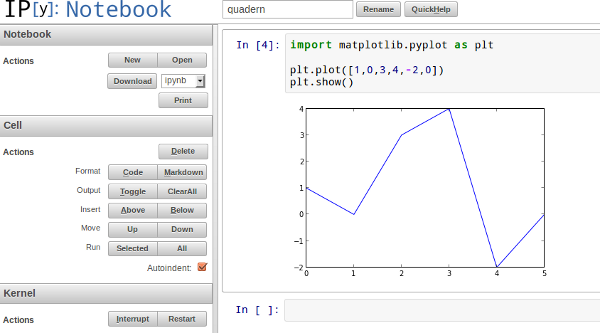
\includegraphics[width=0.9\textwidth]{img/iimage.png}
    \caption{Integració d'imatges a iPython Notebook}
    \label{fig:iimage}
    \end{centering}
\end{figure}




\subsubsection*{Exercici \Roman{exercici}} \stepcounter{exercici}

Graficar la fórmula del sinus i el cosinus utilitzant NumPy i Matplotlib en un quadern de iPython Notebook.





\section{GitHub}

Els nostres quaderns poden ser publicats on-line i compartits a la xarxa. GitHub és un repositori de codi que ens permet compartir arxius i gestionar les versions d'aquests. Podem crear un perfil. Si pugem un quadern a GitHub després podem executar-lo automàticament amb el projecte NBviewer de iPython. Per a pujar els arxius a GitHub primer ens haurem de crear un compte. GitHub és gratuït mentre el nostre treball sigui públic i no excedim certs límits de capacitat. Obrim una terminal

Afegirm l'arxiu al repositori.

\begin{blockcode}
$ git add arxiu.ipynb
\end{blockcode}

Especifiquem un missatge a la nova versió del document.

\begin{blockcode}
$ git commit -m "Arxiu de notebook"
\end{blockcode}


Pujem tots els canvis al servidor

\begin{blockcode}
$ git push
\end{blockcode}


Ara tindrem el nostre projecte actualitzat i podrem passam la URL on es troba el nostre fitxer a la pàgina web NBviewer.
